\documentclass{article}

\usepackage[utf8]{inputenc}
\usepackage[french]{babel}
\usepackage[a4paper, left=2cm, right=2cm, top=2.5cm, bottom=2.5cm]{geometry}
\usepackage{amssymb}
\usepackage{amsmath}
\usepackage{graphicx} % pour les images 
\usepackage{listings} % pour intégrer un code R
\usepackage{xcolor} % pour coloriser le code R intégré

\lstset{
	language=R,
	inputencoding=utf8, 
	extendedchars=true,       
	basicstyle=\ttfamily\footnotesize,
	keywordstyle=\color{blue},
	commentstyle=\color{green!50!black},
	stringstyle=\color{red},
	numbers=left,
	numberstyle=\tiny,
	stepnumber=1,
	breaklines=true,
	literate=%
	{é}{{\'e}}1
	{è}{{\`e}}1
	{ê}{{\^e}}1
	{à}{{\`a}}1
	{ù}{{\`u}}1
	{ç}{{\c{c}}}1
}

\title{Étude des valeurs extrêmes univariées}
\author{El Mazzouji Wahel, Mariac Damien, Condamy Fabian} 
\date{\today} 

\begin{document}

\maketitle 
\newpage
\tableofcontents 
\newpage
\section{Introduction} 

Le théorème central limite, formulé par Pierre-Simon de Laplace en 1809, garantit que, sous des conditions raisonnables, la somme normalisée de ces variables suit asymptotiquement une loi normale. Cette convergence est utile pour étudier le comportement \textbf{global} des observations, mais elle ne renseigne pas sur le comportement des valeurs extrêmes.

Il est donc naturel de se demander quelle peut être la convergence en loi de ses valeurs extrêmes. 
\\
Autrement dit, pour \( X = (X_1, ..., X_n) \) un échantillon de variables aléatoires i.i.d , on pose :


\[
M_n = \max\{X_i \mid i \in \{1, ..., n\} \}
\]

et on s'intéresse à la convergence de \( M_n \), ainsi qu'aux hypothèses sous lesquelles cette convergence a lieu.
\\
\\
\\
Remarque : Etudier le minimum est totalement analogue dans ce qui suit.

\section{Lois de $M_n$}

\subsection{Quelque notation }

On commence par faire une remarque sur la fonction de repartion de $M_n$ en utilisant le fait que les $X_i$ sont i.i.d :
\\
En effet,
\[
F_{M_n}(t) = \mathbb{P}(M_n < t) = \mathbb{P}(X_1 < t,...,X_n <t)=\mathbb{P}(X_1<t)^n = F_{X_1}^n(t) 
\]
\\
Dans la suite, on notera $F(t)$, la fonction de repartition des $X_i$.
\\
\\
Mais on rencontre un probleme ici, puisque si $n\to + \infty$, $F(t)^n$ converge vers 0 (ou 1 si t est la borne sup du support des $X_i$).
\\
\\
\\
L'idée est donc d'introduire 2 suites ($b_n$) et ($a_n$) (avec $a_n > $  0 pour tout n) afin de pouvoir contrôler $M_n$.

Puis étudier la loi de la limite de $\frac{M_n - b_n}{a_n}$. Comme la fonction de repartition caracterise la loi, il nous suffit d'étudier la fonction $G$ définie pour tout t dans le support des $X_i$ comme :

\[
\mathbb{P} \left( \frac{M_n - b_n}{a_n} < t \right) \xrightarrow[n\to +\infty]{} G(t)
\]

à ce stade la, il nous faut donc trouver toutes les distributions G qui peuvent apparaître comme limite dans l’équation ci-dessus.
\\
\\
Pour ce faire, nous allons utiliser le théoreme suivant : 
\\
\\
\underline{\textbf{Théorème}:}
Soit \( Y_n \) une variable aléatoire de fonction de répartition \( F_n \), et soit \( Y \) une variable aléatoire de fonction de répartition \( F \).  
Alors $Y_n \xrightarrow{\mathcal{L} } Y$ si et seulement si pour toute fonction $z$ réelle, bornée et continue :
\[
\mathbb{E}[z(Y_n)] \to \mathbb{E}[z(Y)].
\]

En prenant ici $Y_n = \frac{M_n -b_n}{a_n}$, on obtient :
\[
\mathbb{E}[z(\frac{M_n -b_n}{a_n})] = \int_{-\infty}^{\infty} z(\frac{x-b_n}{a_n}) \: n \:  F^{n-1} (x)dF(x)
\]

L'astuce ici va être de faire un changement de variable astucieux. On va poser : 

\[
x = Q(1-\frac{1}{y}) = K(y) \; \; \; \; \; \; \text{avec Q la fonction quantile}
\]

\begin{equation}\label{eq:1.1}
    \text{Donc,} \; \; \int_{-\infty}^{\infty} z\Bigl(\frac{x-b_n}{a_n}\Bigr) \, n \, F^{n-1}(x)\,dF(x)
    =\int_{0}^{n} z\Bigl(\frac{K\Bigl(\frac{n}{v}\Bigr)-b_n}{a_n}\Bigr)
    \Bigl(1-\frac{v}{n}\Bigr)^{n-1}dv.
\end{equation}
\\
\\
Or, on a $\lim_{n \to \infty} ( 1 - \frac{v}{n})^{n-1} = e^{-v}$ , et on a $\lim_{n \to \infty} \int_{0}^{n} = \int_{0}^{+ \infty}$.

\subsection{Paramètre $b_n$}

On en déduit une bonne valeur pour $b_n$. En effet,
\[
\mathbb{P} \left( \frac{M_n - b_n}{a_n} < t \right) \xrightarrow[n\to +\infty]{} G(t) \in ]0:1[
\]
\[
\Longleftrightarrow F^n(a_n t + b_n) \xrightarrow[n\to +\infty]{} G(t)
\]
\[
\Longleftrightarrow n \: ln(F(a_n t + b_n)) \xrightarrow[n\to +\infty]{} ln(G(t))
\]
\[
\Longleftrightarrow n(- F(a_n t + b_n) + 1) \xrightarrow[n\to +\infty]{} ln(G(t))
\]
\[
\Longleftrightarrow n \: \mathbb{P}(X_1 > a_n t + b_n ) \xrightarrow[n\to +\infty]{} - ln(G(t))
\]
On obtient alors pour paramètre d'échelle :
\[
n \mathbb{P}(X_1 > b_n) =1  \Longleftrightarrow \mathbb{P}(X_1 < b_n) = 1 - \frac{1}{n}
\]
\[
\Longleftrightarrow F(b_n) = 1 - \frac{1}{n}
\]
\[
b_n = Q(1-\frac{1}{n}) = K(n)
\]
Dans la dernière équivalence, on a composé par la fonction quantile (qui est bien définie pour chaque distribution)
\\
\subsection{Paramètre $a_n$}
Avec le parametre $b_n$ définie au dessus, on obtient alors une condition (C), il faut qu'il existe une fonction $a$ tel que $\lim_{x \to \infty} \frac{K(\frac{x}{v}) - K(x)}{a(x)}$ converge (vers une fonction $h(n)$). 
\\
\\
\textbf{Proposition :}
\\
Les limites possibles sont données par :

\begin{equation}\label{eq:1.2}
    c\,h_{\gamma}(u) 
    \;=\; 
    c \int_{1}^{u} v^{-\gamma - 1}\,dv 
    \;=\; 
    c\,\frac{u^{\gamma} - 1}{\gamma}.
\end{equation}

Nous interprétons $h_{0}(u) = \log(u)$ lorsque $\gamma = 0$.*
\\
\\
\; On ne veut pas que $c=0$, car il conduit à une limite dégénérée pour $\frac{X_{n,n} - b_n}{a_n}$. 
Ensuite, le cas $c>0$ peut être ramené au cas $c=1$ en incorporant $c$ dans la fonction $a$. 

Nous remplaçons la condition $(C)$ par une condition plus informative, appelée 
"\textit{condition extrémale du domaine d’attraction}" :
\[
\lim_{x\to \infty} \frac{U(xu) - U(x)}{a(x)} 
\;=\; 
h_{\gamma}(u), 
\quad 
\text{pour } u>0.
\]
Ceci indique que les limites possibles sont essentiellement décrites par la \textit{famille à un paramètre} $h_{\gamma}$. 
\\
\\
\\
\textbf{Preuve de la Proposition}  
\\
Soient $u,v > 0$. Alors :
\[
\frac{U(xuv) - U(x)}{a(x)} 
\;=\; 
\frac{U(xuv) - U(xu)}{a(xu)} \,\frac{a(xu)}{a(x)}
\;+\;
\frac{U(xu) - U(x)}{a(x)}.
\tag{2.3}
\]
Si la limite dans $(C)$ est satisfaite, alors le rapport $\frac{a(ux)}{a(x)}$ converge vers g(u).
\\
De plus, pour $u,v>0$,
\[
\frac{a(xuv)}{a(x)} 
\;=\;
\frac{a(xuv)}{a(xv)} \,\frac{a(xv)}{a(x)}.
\]
Par passage à la limite (pour x), la fonction $g$ satisfait l'\textit{équation fonctionnelle de Cauchy} :
\[
g(uv) = g(u)\,g(v).
\]
\\
Les solutions de cette équation sont de la forme $g(u)= u^{\gamma}$ avec $\gamma$ un réel.
\\
Donc, $a$ est une fonction à variation régulière c'est à dire qu'on a $\lim_{x\to \infty} \frac{a(ux)}{a(x)} \;=\; x^{\gamma} l(x)$
\\
\\
\subsection{Les lois limites}
En reprenant $(2.3)$ et en utilisant ce qui précède, on obtient :
\[
\lim_{x\to \infty} \frac{U(xuv) - U(x)}{a(x)} = u^{\gamma} h(v) + h(u)
\]
\[
\text{autrement dit :} \; \; h_{\gamma}(uv)= h_{\gamma}(u) + h_{\gamma}(v)
\]
\\
\\
On fait alors une disjonction de cas sur la valeur de gamma.
\\
\subsubsection{1. Cas \(\gamma\neq0\)}

En reprenant l'équation \eqref{eq:1.2}, on obtient :
\[
h_\gamma\Bigl(\frac{1}{v}\Bigr)=\frac{(1/v)^\gamma-1}{\gamma}=\frac{v^{-\gamma}-1}{\gamma}.
\]
Posons \(u=\frac{v^{-\gamma}-1}{\gamma}\). On résout alors pour \(v\) :
\[
v^{-\gamma}=1+\gamma u\quad\Longrightarrow\quad v=(1+\gamma u)^{-1/\gamma}.
\]
On définit ainsi la fonction
\[
\eta_\gamma(u)=(1+\gamma u)^{-1/\gamma}.
\]
Le changement de variable de \(v\) à \(u\) permet de réécrire l'intégrale limite sous la forme
\[
\int_{u\in S_\gamma} z(u)\,d\Bigl\{\exp\Bigl[-\eta_\gamma(u)\Bigr]\Bigr\},
\]
ce qui conduit à identifier la loi limite par
\[
G_\gamma(u)=\exp\Bigl\{-\eta_\gamma(u)\Bigr\}=\exp\Bigl\{-\left(1+\gamma u\right)^{-1/\gamma}\Bigr\}.
\]
La nature du support \(S_\gamma\) dépend du signe de \(\gamma\) :
\begin{itemize}
    \item Si \(\gamma>0\), l'inversion montre que \(v\in(0,1)\) correspond à \(u>-\frac{1}{\gamma}\) (loi de Fréchet).
    \item Si \(\gamma<0\), on trouve que \(u<-\frac{1}{\gamma}\) (loi de Weibull).
\end{itemize}
\subsubsection{2. Cas \(\gamma=0\)}
Lorsque \(\gamma\to0\), la fonction \(h_\gamma\) tend par continuité vers
\[
h_0(u)=\ln u.
\]
De même, le changement de variable s'adapte : 
\[
u=h_0\Bigl(\frac{1}{v}\Bigr)=\ln\Bigl(\frac{1}{v}\Bigr)=-\ln v,
\]
ce qui implique
\[
v=e^{-u}.
\]
Le changement de variable transforme alors l'intégrale limite en
\[
\int_{-\infty}^{\infty} z(u)\,d\Bigl\{\exp\Bigl[-e^{-u}\Bigr]\Bigr\},
\]
et la loi limite est alors donnée par
\[
G_0(u)=\exp\Bigl\{-e^{-u}\Bigr\},\qquad u\in\mathbb{R},
\]
ce qui correspond à la loi de Gumbel.
\\
\subsection{Résumé}
Les lois limites qui s'imposent dependent d'un parametre $\gamma$ et sont les suivantes :
\\
\begin{itemize}
    \item \textbf{Si \(\gamma>0\)} (loi de Fréchet) :
    \[
    G_\gamma(u)=\exp\left\{-\left(1+\gamma u\right)^{-1/\gamma}\right\}, \quad u > -\frac{1}{\gamma}.
    \]
    
    \item \textbf{Si \(\gamma=0\)} (loi de Gumbel) :
    \[
    G_0(u)=\exp\left\{-e^{-u}\right\}, \quad u\in\mathbb{R}.
    \]
    
    \item \textbf{Si \(\gamma<0\)} (loi de Weibull) :
    \[
    G_\gamma(u)=\exp\left\{-\left(1+\gamma u\right)^{-1/\gamma}\right\}, \quad u < -\frac{1}{\gamma}.
    \]
\end{itemize}

\section{Quelques exemples numériques}

\noindent Voici maintenant quelques applications numériques sur des lois usuelles de ce que nous avons vu dans cette section. Pour chacune des représentations suivantes, nous avons simulé 1000 fois chaque loi puis ensuite effectué 10000 simulations pour le maximum afin d'avoir une précision correcte.

\subsubsection{Loi uniforme}

\noindent Pour la loi uniforme sur [0,1], on peut montrer théoriquement que la limite du max est une loi exponentielle de paramètre 1. \\
\noindent Avec notre machine, nous obtenons le graphe suivant :

\begin{center}
	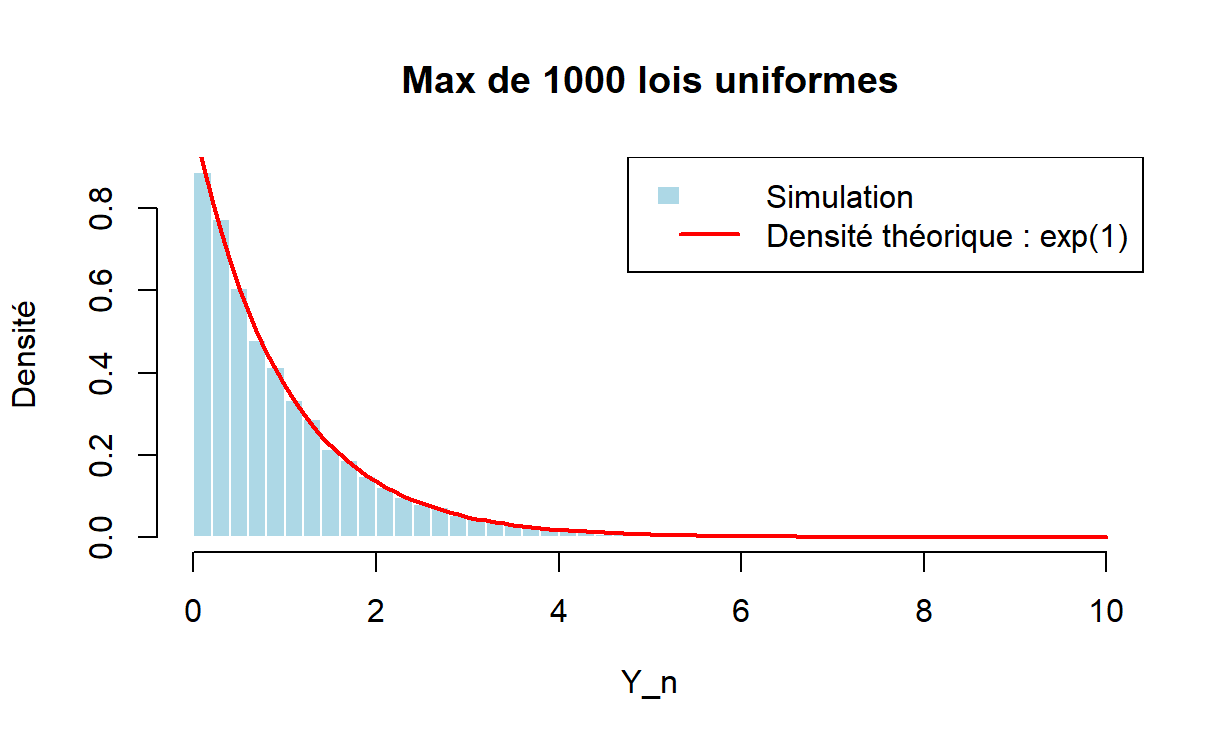
\includegraphics[scale=0.8]{./Codes_R/Max_Uniforme.png} 
\end{center}

\subsubsection{Loi exponentielle}
\noindent Pour une loi exponentielle de paramètre 1, la loi limite est une loi de Gumbel. 

\begin{center}
	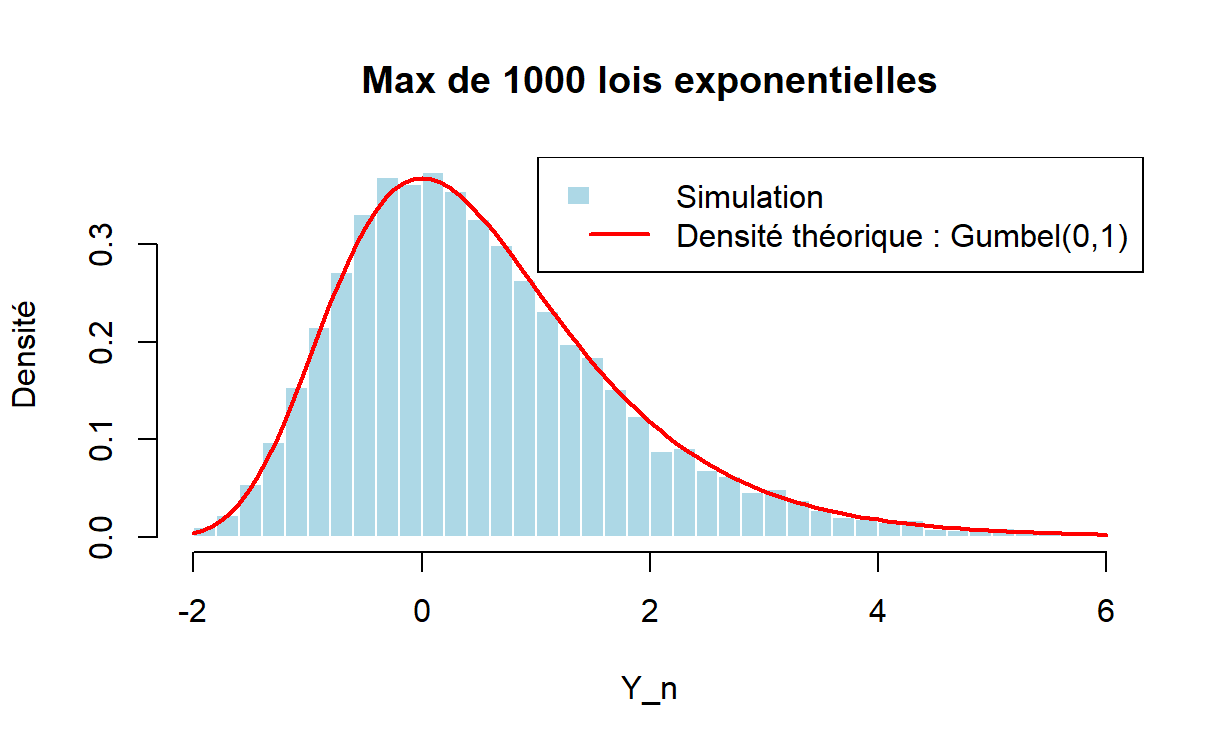
\includegraphics[scale=0.8]{./Codes_R/Max_Expo.png} 
\end{center}


\subsubsection{Loi normale}

\noindent Pour maintenant une loi normale centrée-réduite, on peut montrer que la loi limite est encore une fois une loi de Gumbel.

\begin{center}
	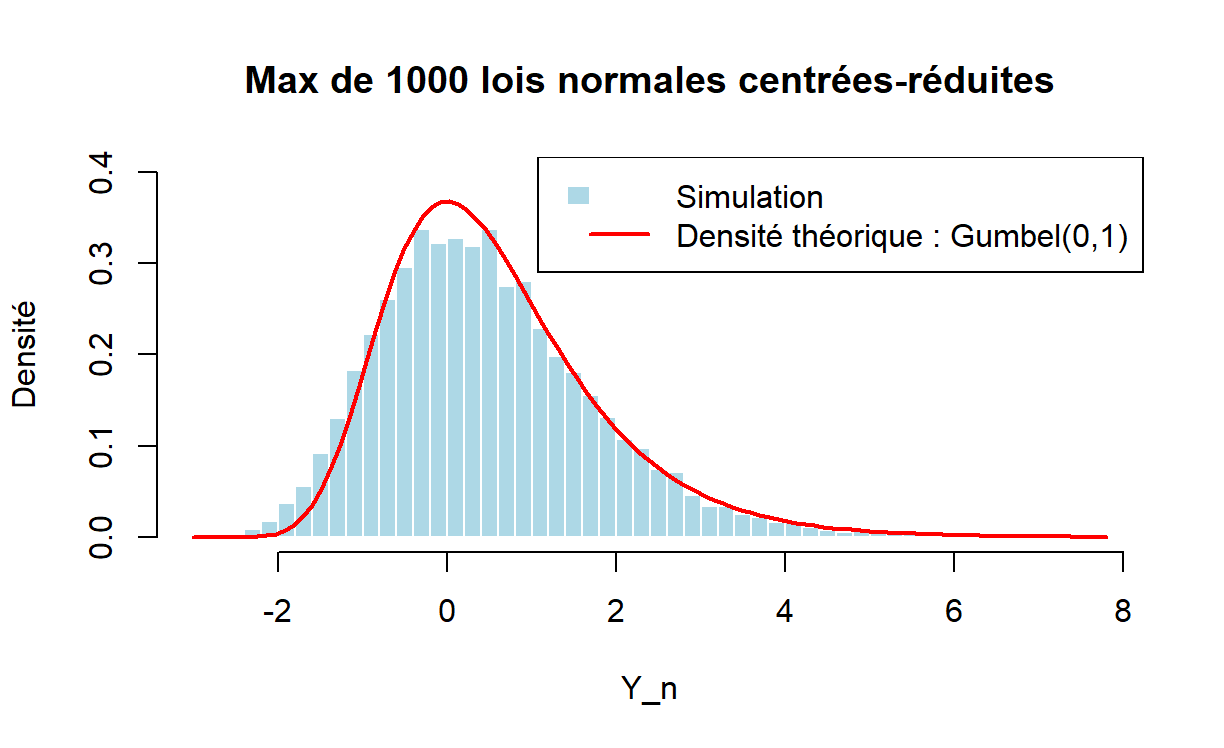
\includegraphics[scale=0.8]{./Codes_R/Max_Normale.png} 
\end{center}

\noindent Notons ainsi que l'on a la même loi limite que pour la loi exponentielle de paramètre 1.

\subsubsection{Loi de Cauchy}

\noindent Enfin, pour une loi de Cauchy (de paramètres 0 et 1 ici), la loi limite est une loi de Fréchet. 

\begin{center}
	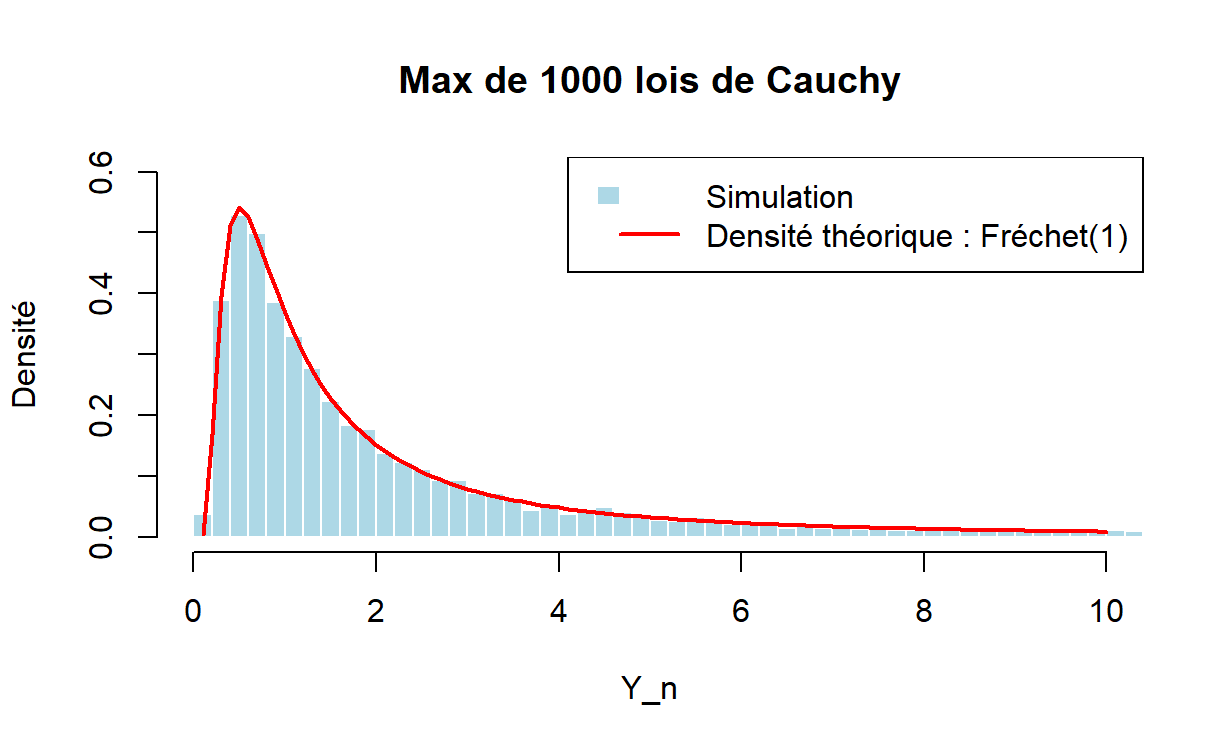
\includegraphics[scale=0.8]{./Codes_R/Max_Cauchy.png} 
\end{center}


\newpage
\section{Estimation du paramètre gamma} 

Soient \(X_1, \dots, X_n\) i.i.d. On définit la fonction de répartition :

\[
F(x) = P(X_1 \leq x), \quad x \in \mathbb{R}
\]

Nous allons définir la fonction de répartition empirique.

\subsection{Fonction de répartition empirique}

\textbf{Définition :} Pour tout \(x \in \mathbb{R}\), la fonction de répartition empirique est donnée par :

\[
F_n(x) = \frac{1}{n} \sum_{i=1}^{n} \mathbb{1}_{(-\infty, x]}(X_i)
\]

où \(\mathbb{1}_{(-\infty, x]}(X_i)\) est l'indicatrice de l'événement \(\{X_i \leq x\}\).
La fonction de répartition empirique utilise la statistique d'ordre.

\subsection{Quantiles et inverse généralisée}

\textbf{Définition :} Soit \(p \in (0,1)\), on appelle \textit{\(p\)-quantile}, noté \(x_p\), de la loi \(F\) toute quantité satisfaisant :

\[
F(x_p) = p
\]

Pour définir un quantile de manière plus générale, on considère l'inverse généralisée de \(F\).

\textbf{Définition :} Pour tout \(u \in [0,1]\), on appelle \textit{inverse généralisée} de \(F\), notée \(F^-\), la fonction définie par :

\[
F^-(u) = \inf \{ x \in \mathbb{R} \mid F(x) \geq u \}
\]

\subsection{Quantiles empiriques}

\textbf{Définition :} Soit \(p \in (0,1)\), on appelle \textit{\(p\)-quantile empirique}, noté \(x_p(n)\), la valeur :

\[
x_p(n) = F_n^-(p) = \inf \{ x \in \mathbb{R} \mid F_n(x) \geq p \}
\]

\subsection{Estimation de \(\gamma\) par la méthode des quantiles}

Pour déterminer les estimateurs de \(\gamma\) pour ces trois distributions, nous utilisons l'estimation par la méthode des quantiles.  
Nous allons commencer par estimer le paramètre \(\gamma\) pour la distribution de Fréchet.

\subsubsection{Rappel de la fonction de répartition}

Rappelons que la fonction de répartition de la loi de Fréchet s'écrit comme :

\[
F(x) = \exp(-x^{-\gamma}), \quad x > 0, \quad \gamma > 0.
\]

On cherche \(x\) tel que :

\[
\exp(-x^{-\gamma}) = p.
\]

En prenant le logarithme, on obtient :

\[
\ln(p) = -x^{-\gamma}
\]

\[
x^{\gamma} = -\frac{1}{\ln(p)}
\]

\subsubsection{Estimation de \(\gamma\) à partir du quantile médian}

On utilise l'estimateur du quantile avec la médiane de la distribution (\(x_{1/2}\)) :

\[
x_{1/2} = (\ln 2)^{-1/\gamma} = f(\gamma),
\]

où \(f(\gamma)\) est une fonction bijective.  
Si l'on sait estimer \(x_{1/2}\), alors on peut facilement estimer \(\gamma\) en inversant \(f\) :

\[
\gamma = f^{-1}(x_{1/2}).
\]

On résout :

\[
x = f(\gamma) \iff x = (\ln 2)^{-1/\gamma}
\]

\[
\iff (\ln 2)^{1/\gamma} = \frac{1}{x}
\]

\[
\iff \frac{1}{\gamma} \ln (\ln 2) = \ln \left(\frac{1}{x}\right) = -\ln x.
\]

D'où :

\[
\gamma = -\frac{\ln (\ln 2)}{\ln x} = f^{-1}(x).
\]

\subsubsection{Convergence et estimation empirique}

Rappelons que le quantile empirique converge en probabilité vers le quantile théorique :

\[
x_p(n) \xrightarrow{\mathbb{P}} x_p = F^{-1}(p).
\]

En particulier, pour \(p = \frac{1}{2}\) :

\[
x_{1/2}(n) \xrightarrow{\mathbb{P}} x_{1/2},
\]

où \(x_{1/2}(n)\) est le quantile empirique d'ordre \(1/2\) (médiane empirique).  

Or, la convergence en probabilité est stable par transformation continue, d'où :

\[
f^{-1}(x_{1/2}(n)) \xrightarrow{\mathbb{P}} f^{-1}(x_{1/2}) = \gamma.
\]

Ainsi, 

\[
\gamma = f^{-1}(x_{1/2}(n))
\]

est un estimateur convergent de \(\gamma\).  
Finalement, l'estimateur de \(\gamma\) est donné par :

\[
\hat{\gamma} = -\frac{\ln (\ln 2)}{\ln x_{1/2}(n)}.
\]
\subsection{Estimation de \(\gamma\) pour la distribution de Gumbel}

La fonction de répartition de Gumbel est donnée par :

\[
F(x) = \exp(-\exp(-x/\gamma)).
\]

Ainsi, pour \(p = \frac{1}{2}\), on a :

\[
F(x_{1/2}) = \frac{1}{2}
\]

\[
\iff \exp(-\exp(-x_{1/2}/\gamma)) = \frac{1}{2}
\]

\[
\iff -\exp(-x_{1/2}/\gamma) = -\ln(2)
\]

\[
\iff \exp(-x_{1/2}/\gamma) = \ln(2)
\]

\[
\iff -\frac{x_{1/2}}{\gamma} = \ln(\ln(2))
\]

\[
\iff \gamma = -\frac{x_{1/2}}{\ln(\ln(2))} = f(x_{1/2}),
\]

où \(f\) est une fonction continue.

\subsubsection{Convergence et estimation empirique}

En utilisant le quantile empirique, on a :

\[
x_{1/2}(n) \xrightarrow{\mathbb{P}} x_{1/2}.
\]

Puisque la convergence en probabilité est stable par transformation continue, il en résulte :

\[
f(x_{1/2}(n)) \xrightarrow{\mathbb{P}} \gamma = f(x_{1/2}).
\]

Ainsi, un estimateur convergent de \(\gamma\) est donné par :

\[
\hat{\gamma} = f(x_{1/2}(n)) = -\frac{x_{1/2}(n)}{\ln(\ln(2))}.
\]

\subsection{Estimation de \(\gamma\) pour la distribution de Weibull}

Ainsi, l'estimateur \(\hat{\gamma}\) est un estimateur convergent de \(\gamma\).

La fonction de répartition de Weibull est donnée par :

\[
F(x) = 1 - \exp(-x^{\gamma}).
\]

Pour \(p = \frac{1}{2}\), nous avons :

\[
F(x_{1/2}) = \frac{1}{2}
\]

\[
\iff 1 - \exp(-x_{1/2}^{\gamma}) = \frac{1}{2}
\]

\[
\iff \frac{1}{2} = \exp(-x_{1/2}^{\gamma})
\]

\[
\iff -\ln(2) = -x_{1/2}^{\gamma}
\]

\[
\iff \ln(2) = x_{1/2}^{\gamma}.
\]

En appliquant le logarithme népérien :

\[
\gamma \ln(x_{1/2}) = \ln(\ln 2)
\]

\[
\iff \gamma = \frac{\ln(\ln 2)}{\ln(x_{1/2})} = \varphi(x_{1/2}),
\]

où \(\varphi\) est une fonction continue.

\subsubsection{Convergence et estimation empirique}

Puisque \(x_{1/2}(n)\) converge en probabilité vers \(x_{1/2}\), on a :

\[
\varphi(x_{1/2}(n)) \xrightarrow{\mathbb{P}} \varphi(x_{1/2}) = \gamma.
\]

Finalement, un estimateur convergent de \(\gamma\) est donné par :

\[
\hat{\gamma} = \frac{\ln(\ln 2)}{\ln(x_{1/2}(n))}.
\]

\section{Méthodes d'estimation de l'indice de valeurs extrêmes}
Dans cette section, nous nous intéressons aux différentes méthodes d'estimation du paramètre \(\gamma\), intervenant dans la distribution des valeurs extrêmes généralisée. D'une part, des approches non paramétriques sont dédiées à l'estimation de l'indice de queue, notamment les estimateurs de Hill et de Pickands. D'autre part, des méthodes paramétriques ont été développées, parmi lesquelles la méthode du maximum de vraisemblance, la méthode des moments et les approches bayésiennes.
\newline
\textbf{Définition :} On appelle \textit{statistique d'ordre} la permutation aléatoire de l'échantillon \(X_1, \dots, X_n\), qui ordonne les valeurs de l’échantillon par ordre croissant :

\[
X_{(1)} \leq X_{(2)} \leq \dots \leq X_{(n)}
\]

En particulier, \(X_{(1)} = \min X_i\) et \(X_{(n)} = \max X_i\).

\textbf{Attention !!!} Même si les \(X_i\) sont i.i.d., les statistiques d’ordre \(X_{(i)}\) ne le sont pas.

\textbf{Définition :} On dit qu'une suite \((k_n)_{n \geq 0}\) d'entiers est intermédiaire si :

\[
\lim_{n \to \infty} k_n = \infty \quad et \lim_{n \to \infty} \frac{k_n}{n} = 0
\]

\textbf{Définition :}
On dit qu'un estimateur \(\hat{\gamma_{n}}\) est convergent s'il converge en probabilité vers \(\gamma\), soit :
\[
\lim_{n \to \infty} P(\lvert \hat{\gamma_{n}} - \gamma \rvert > \epsilon) = 0 \quad \forall \epsilon > 0
\]
\subsection{Estimateur de Pickands}

L'estimateur de Pickands est défini par la statistique 
\[
\hat{\gamma}_{k,n} = \frac{1}{\ln(2)} \ln\left(\frac{X_{k,n} - X_{2k,n}}{X_{2k,n} - X_{4k,n}}\right)
\]

Cet estimateur présente l'avantage d'être applicable quelle que soit la distribution des extrêmes. Cependant, la représentation graphique de cet estimateur en fonction du nombre \(k\) d'observations considérées révèle généralement un comportement volatil au départ, ce qui peut nuire à la lisibilité du graphique. De plus, cet estimateur est particulièrement sensible à la taille de l'échantillon sélectionné, ce qui le rend peu robuste.

Cet estimateur est asymptotiquement normal, avec :
\[
\sqrt{k} \frac{\hat{\gamma_{k,n}} - \gamma}{\sigma(\gamma)} \xrightarrow{\mathcal{L}} \mathcal{N}(0,1)
\]
Lorsque \( k \to +\infty \), la variance asymptotique est donnée par :

\[
\sigma(\gamma)= \frac{\gamma \sqrt{2^{(2\gamma+1)}+1}}{2(2^{\gamma}-1) \ln(2)}
\]

Une généralisation de l'estimateur de Pickands a été introduite comme suit :
\[
\hat{\gamma}_{(k,u,v)} = \frac{1}{\ln(v)} \ln\left(\frac{X_{n-k+1,n} - X_{n-[uk]+1,n}}{X_{n-[vk]+1,n} - X_{n-[uvk]+1,n}}\right)
\]
où \(u\) et \(v\) sont des réels positifs différents de 1, de sorte que les indices \([vk]\), \([uk]\) et \([uvk]\) ne dépassent pas \(n\). Lorsque \(u = v = 2\), on retrouve l'estimateur de Hill \(\hat{\gamma}_{k,n}\).

\subsection{Construction de l'estimateur de Pickands}
\textbf{Proposition :} (Caractérisations de \( D(H_{\gamma}) \))

Pour \( \gamma \in \mathbb{R} \), les affirmations suivantes sont équivalentes. \newline
\( (a) \quad F \in D(H_{\gamma}) \) \newline
\( (b) \) Pour une certaine fonction positive \( c(t) = a\left( \frac{1}{t} \right) \) :

\[
\lim_{t \to 0} \frac{U(tx) - U(t)}{c(t)} = 
\begin{cases} 
\frac{x^\gamma - 1}{\gamma} & \text{si } \gamma \neq 0, \\
\log(x) & \text{si } \gamma = 0, 
\end{cases}
\quad \text{pour } x > 0.
\]
La dernière affirmation est équivalente à :
\[
\lim_{s \to 0} \frac{U(sx) - U(s)}{U(sy) - U(s)} = 
\begin{cases} 
\frac{x^\gamma - 1}{y^\gamma - 1} & \text{si } \gamma \neq 0, \\
\frac{\log(x)}{\log(y)} & \text{si } \gamma = 0.
\end{cases}
\]
pour \(x,y > 0\) et \(y \neq 1\). \newline

\textbf{Lemme A:}
Soit \(X_1, \dots, X_n\) des variables aléatoires indépendantes et de fonction de répartition \(F\).
Soit \(U_1, \dots, U_n\) des variables aléatoires indépendantes de loi uniforme \(\left[0,1\right]\). Alors \(F^{-1}(U_{1,n}), \dots, F^{-1}(U_{n,n})\) a même loi que \((X_{1,n}, \dots, X_{n,n})\)\newline
\textbf{Preuve de la construction de l'estimateur de Pickands :}

On déduit de la proposition précédente que pour $\gamma \in \mathbb{R}$ et $\alpha$ on a avec le choix $t = 2s$, $x = 2$ et $y = \frac{1}{2}$,
\[
\lim_{t \to \infty} \frac{U(t) - U(t/2)}{U(t/2) - U(t/4)} = 2^{\gamma}.
\]

En fait, en utilisant la croissance de $U$ qui se déduit de la croissance de $F$, on obtient
\[
\lim_{t \to \infty} \frac{U(t) - U(t_{c_1}(t))}{U(t_{c_1}(t)) - U(t_{c_2}(t))} = 2^{\gamma}
\]
dès que $\lim_{t \to \infty} c_1(t) = \frac{1}{2}$ et $\lim_{t \to \infty} c_2(t) = \frac{1}{4}$. Il reste donc à trouver des estimateurs pour $U(t)$.

Soit $k(n), n \geq 1$ une suite d’entiers telle que $1 \leq k(n) \leq \frac{n}{4}$ et $\lim_{n \to \infty} \frac{k(n)}{n} = 0$ et $\lim_{n \to \infty} k(n) = \infty$.

Soit $(V_{1,n},\dots,V_{n,n})$ la statistique d’ordre d’un échantillon de variables aléatoires indépendantes de loi de Pareto. On note $F_V(x) = 1 - x^{-1}, x \geq 1$.

On déduit avec certains résultats de bases liés à $(V_{1,n},\dots,V_{n,n})$ que les suites
\[
\frac{k}{n} V_{n-k+1,n}, \quad \frac{2k}{n} V_{n-2k+1,n}, \quad \frac{4k}{n} V_{n-4k+1,n}
\]
pour \(n \geq 1\) convergent en probabilité vers 1.

On en déduit en particulier, les convergences en probabilité suivantes :
\[
V_{n-k+1,n}  \to \infty, \quad \frac{V_{n-2k+1,n}}{V_{n-k+1,n}} \to \frac{1}{2}, \quad \frac{V_{n-4k+1,n}}{V_{n-k+1,n}} \to \frac{1}{4}.
\]

Donc la convergence suivante a lieu en probabilité :
\[
\frac{U(V_{n-k+1,n}) - U(V_{n-2k+1,n})}{U(V_{n-2k+1,n}) - U(V_{n-4k+1,n})} \to 2^{\gamma}.
\]

Remarquons que si $x \geq 1$, alors $U(x) = F^{-1}(F_V(x))$. On a donc
\[
(U(V_{1,n}), \dots, U(V_{n,n})) = (F^{-1}(F_V(V_{1,n})), \dots, F^{-1}(F_V(V_{n,n}))).
\]

Or \(F_V\) est la fonction de répartition de la loi de Pareto. \newline
On déduit de la croissance de $F_V$ que $(F^{-1}(F_V(V_{1,n})),\dots, F^{-1}(F_V(V_{n,n})))$ a la même loi qu’une suite de $n$ variables aléatoires uniformes sur $[0,1]$ indépendantes. 

On déduit du lemme A que le vecteur aléatoire $(F^{-1}(F_V(V_{1,n})),\dots, F^{-1}(F_V(V_{n,n})))$ a la même loi que $(X_1,\dots,X_n)$. 

Donc la variable aléatoire \(\frac{U(V_{n-k+1,n}) - U(V_{n-2k+1,n})}{U(V_{n-k+1,n}) - U(V_{n-4k+1,n})}\) a la même loi que :

\[
\frac{X_{n-k+1,n} - X_{n-2k+1,n}}{X_{n-k+1,n} - X_{n-4k+1,n}}
\]

Ainsi cette quantité converge en loi vers $2^{\gamma}$ quand $n$ tend vers l’infini.

\subsection{Estimateur de Hill}

Tout d'abord, l'estimateur de Hill est applicable uniquement aux distributions de Fréchet (\(\gamma > 0\)), où il permet d'obtenir un estimateur de l'indice de queue plus efficace que celui de Pickands. Cet estimateur est défini par la statistique suivante :
\[
\hat{\gamma}_{k,n} = \frac{1}{k} \sum_{i=1}^{k} \ln(\frac{X_{n-i+1,n}}{X_{n-k,n}})
\]
pour \( k \in \{1, \dots, n-1\} \).
Si l'on choisit \( k, n \to +\infty \), de sorte que \(\frac{k}{n} \to 0\), alors on peut montrer que \(\lim_{k \to \infty} \hat{\gamma}_{k,n} = \gamma\). Cet estimateur possède la propriété d'être asymptotiquement normal, ce qui signifie que :

\[
\sqrt{k} \frac{\hat{\gamma}_{k,n} - \gamma}{\gamma} \xrightarrow{\mathcal{L}} \mathcal{N}(0,1)
\]

Il existe plusieurs approches pour construire l'estimateur de Hill. Une approche possible consiste à utiliser la méthode du maximum de vraisemblance. 

Tout d'abord, on considère une suite de variables aléatoires \( X_1, \dots, X_n \) i.i.d. suivant une loi de Pareto de paramètre \( \lambda > 0 \), dont la fonction de répartition est donnée par :  

\[
F(x) = 1 - x^{-\lambda}, \quad \text{pour } x \geq 1.
\]

La densité de probabilité associée est alors :

\[
f(x) = \lambda x^{-\lambda - 1}, \quad \text{pour } x \geq 1.
\]

La fonction de vraisemblance est donnée par :

\[
L(x_1, \dots, x_n, \lambda) = \prod_{i=1}^{n} f(x_i) = \lambda^{n} \prod_{i=1}^{n} x_i^{-\lambda - 1}.
\]

En prenant le logarithme, on obtient la log-vraisemblance :

\[
\log L(x_1, \dots, x_n, \lambda) = n \log \lambda - (\lambda + 1) \sum_{i=1}^{n} \log x_i.
\]

En dérivant cette expression par rapport à \( \lambda \), on obtient :

\[
\frac{d \log L}{d \lambda} = \frac{n}{\lambda} - \sum_{i=1}^{n} \log x_i.
\]

En dérivant une seconde fois, nous obtenons :

\[
\frac{d^2 \log L}{d \lambda^2} = -\frac{n}{\lambda^2} < 0,
\]

ce qui confirme qu'il s'agit bien d'un maximum.  

Ainsi, l'estimateur du maximum de vraisemblance de \( \frac{1}{\lambda} \) est donné par :

\[
\hat{\lambda}^{-1} = \frac{1}{n} \sum_{i=1}^{n} \log X_i.
\]

Cela implique que l'estimateur du paramètre \( \lambda \) est :

\[
\hat{\lambda} = \left( \frac{1}{n} \sum_{i=1}^{n} \log X_i \right)^{-1}.
\]

\subsection{Estimateur de DEDH}
Le troisième estimateur de l'indice de queue est celui proposé par Dekkers, Einmahl et De Haan. Il s'agit d'une généralisation de l'estimateur de Hill, applicable à tous les domaines d'attraction. Il est défini par :

\[
\hat{\gamma}_n^{(DEdH)}(k_n) = \mathcal{M}^{(1)}_{k_n} + 1 - \frac{1}{2} \left( 1 - \frac{(\mathcal{M}^{(1)}_{k_n})^2}{\mathcal{M}^{(2)}_{k_n}} \right)^{-1}
\]

où 
\[
\mathcal{M}^{(r)}_{k_n} = \frac{1}{k_n} \sum_{i=1}^{k_n} (\ln(X_{(n-i+1)}) - \ln(X_{(n-k_n)}))^r.
\]
La valeur de \(\mathcal{M}^{(1)}_{k_n}\) correspond à l'estimateur de Hill.

L'estimateur de DEDH possède la propriété de convergence en loi :

\[
\sqrt{k_n}(\frac{\hat{\gamma}_n^{(DEdH)}(k_n) - \gamma}{\sigma_M}) \xrightarrow{\mathcal{L}} \mathcal{N}(0,1) \quad \text{quand } n \to \infty.
\]

où :

\[
\sigma_M^2 = 
\begin{cases} 
1 + \gamma^2, & \text{si } \gamma \geq 0, \\ 
(1 - \gamma^2)(1 - 2\gamma)
\left( 4 - \frac{8 (1 - 2\gamma)}{1 - 3\gamma} - \frac{(5 - 11\gamma)(1 - 2\gamma)}{(1 - 3\gamma)(1 - 4\gamma)} \right), 
& \text{si } \gamma < 0.
\end{cases}
\]

En pratique, il est difficile de comparer ces estimateurs de manière tranchée. Toutefois, l'estimateur de Hill se distingue par une variance asymptotique plus faible, ce qui justifie son choix dans la suite. Étant donné que cet estimateur n'est valide uniquement pour les distributions appartenant au domaine d'attraction de Fréchet, c'est-à-dire dans le cas où \(\gamma > 0\), il est essentiel de vérifier cette hypothèse. 

\section{Sélection des estimateurs de l'indice de valeurs extrêmes}

Le choix de l’estimateur dépend du type de distribution sous-jacente. L’estimateur de Hill est spécifiquement adapté aux distributions de Fréchet (\(\gamma > 0\)), caractérisées par des queues lourdes. Il est donc plus efficace dans ce cas et sera préféré à l’estimateur de Pickands.  

Cependant, pour les distributions de Weibull (\(\gamma < 0\)) et Gumbel (\(\gamma = 0\)), l’estimateur de Hill n’est pas applicable. Dans ces cas, on utilise l’estimateur de Pickands, qui est valide quel que soit le signe de \( \gamma \).  

L'estimateur de Pickands est basé sur les distances entre deux statistiques d'ordre, sans tenir compte du maximum de l’échantillon, ce qui entraîne une perte d'information sur la queue de distribution. Par conséquent, il présente une plus grande volatilité que l'estimateur de Hill, qui repose sur la moyenne des logarithmes des observations.

\section{Détermination du domaine d'attraction}
Une approche graphique qui permet de déterminer à quel domaine d'attraction appartiennent les données consiste à tracer le quantile plot généralisé repris de Anis Borchani (2010). Le quantile plot généralisé est défini par :
\[
\left( \ln\left( \frac{n+1}{j} \right), \ln\left( \hat{\gamma}_{j,n}^{(UH)} \right) \right) \quad \text{pour tout } j \in \left[ 1; k_n \right]
\]
avec 
\[
\hat{\gamma}_{j,n}^{(UH)} = X_{(n-j)} \hat{\gamma}_{n}^{(H)}(k_n).
\]
La difficulté pratique dans le calcul de ces estimateurs réside dans le choix du nombre d'excès \(k_n\) à prendre en compte. Si les estimateurs sont calculés en utilisant un trop grand nombre d'observations, leur biais sera élevé. À l'inverse, si le nombre d'observations est trop faible, cela entraînera une variance importante.

\section{Annexe}

\subsection{Codes R}

\noindent Voici un exemple de code R utilisé dans la première section :

\begin{lstlisting}
	# Paramètres
	n <- 1000        # Taille de l'échantillon pour la simulation des lois uniformes
	N <- 10000       # Nombre de simulations pour le maximum
	
	# Simulation des maxima de lois uniformes(0,1)
	set.seed(123)    # fixation de l'aléa
	M_n <- replicate(N, max(runif(n))) # M_n = max / X_n = runif
	
	# Normalisation pour observer la convergence
	Y_n <- n * (1 - M_n)
	
	# Histogramme des valeurs transformées
	hist(Y_n, breaks = 50, probability = TRUE, 
	col = "lightblue", border = "white", ylab = "Densité",
	xlab = expression(Y_n), main = "Max de 1000 lois uniformes")
	
	# Densité théorique de la loi exponentielle (paramètre = 1)
	curve(dexp(x, rate = 1), col = "red", lwd = 2, add = TRUE)
	
	# Légende
	legend("topright", legend = c("Simulation", "Densité théorique : exp(1)"),
	fill = c("lightblue", NA), border = c("white", NA), 
	lty = c(NA, 1), col = c(NA, "red"), lwd = c(NA, 2))
\end{lstlisting}
\end{document}